% metadata.tex
\def\documentTitle{Preliminary Design Report}
\def\documentTeam{CDOSR (CoderDojo Oradea Space Robotics)}
\def\documentOrganization{CoderDojo Oradea}
\def\documentCountry{Romania}
\def\documentVersion{1.0}
\def\documentDate{\today}
\def\documentCompetition{Romanian CanSat Competition 2025}
% Define all input paths
\makeatletter
\def\input@path{%
  {./styles/}%
  {./content/appendices/}%
  {./content/sections/}%
  {./content/sections/section_1/}%
  {./content/sections/section_2/}%
  {./content/sections/section_4/}%
  {./content/sections/section_5/}%
  {./content/sections/section_6/}%
  {./content/sections/section_7/}%
}
\makeatother

% Define commands for importing from specific sections
\newcommand{\inputSectionOne}[1]{\input{./content/sections/section_1/#1}}
\newcommand{\inputSectionTwo}[1]{\input{./content/sections/section_2/#1}}
\newcommand{\inputSectionThree}[1]{\input{./content/sections/section_3/#1}}
\newcommand{\inputSectionFour}[1]{\input{./content/sections/section_4/#1}}
\newcommand{\inputSectionFive}[1]{\input{./content/sections/section_5/#1}}
\newcommand{\inputSectionSix}[1]{\input{./content/sections/section_6/#1}}
\newcommand{\inputSectionSeven}[1]{\input{./content/sections/section_7/#1}}
\newcommand{\inputAppendix}[1]{\input{./content/appendices/#1}}

\documentclass[11pt]{article}
\usepackage{CDOSR_CanSat}
% \usepackage{./styles/CDOSR_CanSat}
% \usepackage{CDOSR_Headers}
\usepackage{./styles/CDOSR_Headers}
% acronyms.tex
\usepackage[acronym,toc,nogroupskip]{glossaries}
\makeglossaries

% Technical acronyms
\newacronym{pdr}{PDR}{Preliminary Design Report}
\newacronym{cdr}{CDR}{Critical Design Review}
\newacronym{imu}{IMU}{Inertial Measurement Unit}
\newacronym{pcb}{PCB}{Printed Circuit Board}
\newacronym{rf}{RF}{Radio Frequency}
\newacronym{sipm}{SiPM}{Silicon Photomultiplier}
\newacronym{uart}{UART}{Universal Asynchronous Receiver-Transmitter}
\newacronym{i2c}{I2C}{Inter-Integrated Circuit}
\newacronym{spi}{SPI}{Serial Peripheral Interface}
\newacronym{gps}{GPS}{Global Positioning System}
\newacronym{lora}{LoRa}{Long Range radio}
\newacronym{gsm}{GSM}{Global System for Mobile Communications}
\newacronym{rtos}{RTOS}{Real-Time Operating System}

% Technical terms
\newglossaryentry{muon}{
  name={muon},
  description={A subatomic particle similar to an electron but with much greater mass, produced when cosmic rays interact with the Earth's atmosphere},
  plural={muons}
}

\newglossaryentry{telemetry}{
  name={telemetry},
  description={The process of recording and transmitting the readings of an instrument to a remote location}
}

% \usepackage{xcolor}
% \usepackage{colortbl}
% \usepackage{pgfplots}
% Define colors based on score
\definecolor{high}{RGB}{144, 238, 144}  % Light green for high scores
\definecolor{medium}{RGB}{255, 223, 128} % Light orange for medium scores
\definecolor{low}{RGB}{255, 153, 153}    % Light red for low scores

% Function for cell coloring
\newcommand{\cellcolorbasedonvalue}[1]{
    \ifnum#1>4 \cellcolor{high}#1
    \else\ifnum#1=4 \cellcolor{medium}#1
    \else\cellcolor{low}#1
    \fi\fi
}


% document_settings.tex
% Document-specific settings
\setlength{\headheight}{36.58205pt}
\addtolength{\topmargin}{-24.58205pt}

% Set desired section numbering depth
\setcounter{secnumdepth}{3}
\setcounter{tocdepth}{3}

% Set up headers and footers
\fancyhf{}
\fancyhead[L,R]{\thepage}
\fancyhead[R]{\textbf{\leftmark}}
\fancyhead[LO]{\textbf{\rightmark}}

% Set default image paths
\graphicspath{{images/}{images/template/}{images/diagrams/}{images/photos/}{icons/}{images/cdr/}{images/pdr/}}

\title{\documentTitle}
\author{Team: \documentTeam}
\date{\documentDate}

\begin{document}

\cansattitle{\documentTitle}{img_CDOSR.png}{img_CANSAT_RO.png}




\tableofcontents
\clearpage
% \pagestyle{cdosrpage}

\newpage
\inputSection{1}{section_1}
\inputSection{2}{section_2}
% \inputSection{3}{section_3}
\inputSection{4}{section_4}
\inputSection{5}{section_5}
\inputSection{6}{section_6}
\inputSection{7}{section_7}

\theendnotes

% \addbibresource{bibliography.bib}
% \printbibliography

\appendix
\newpage

\appendix
\addcontentsline{toc}{section}{Appendices}
\section*{Appendices}
\section{Time Management - Gantt Chart}\label{A1} 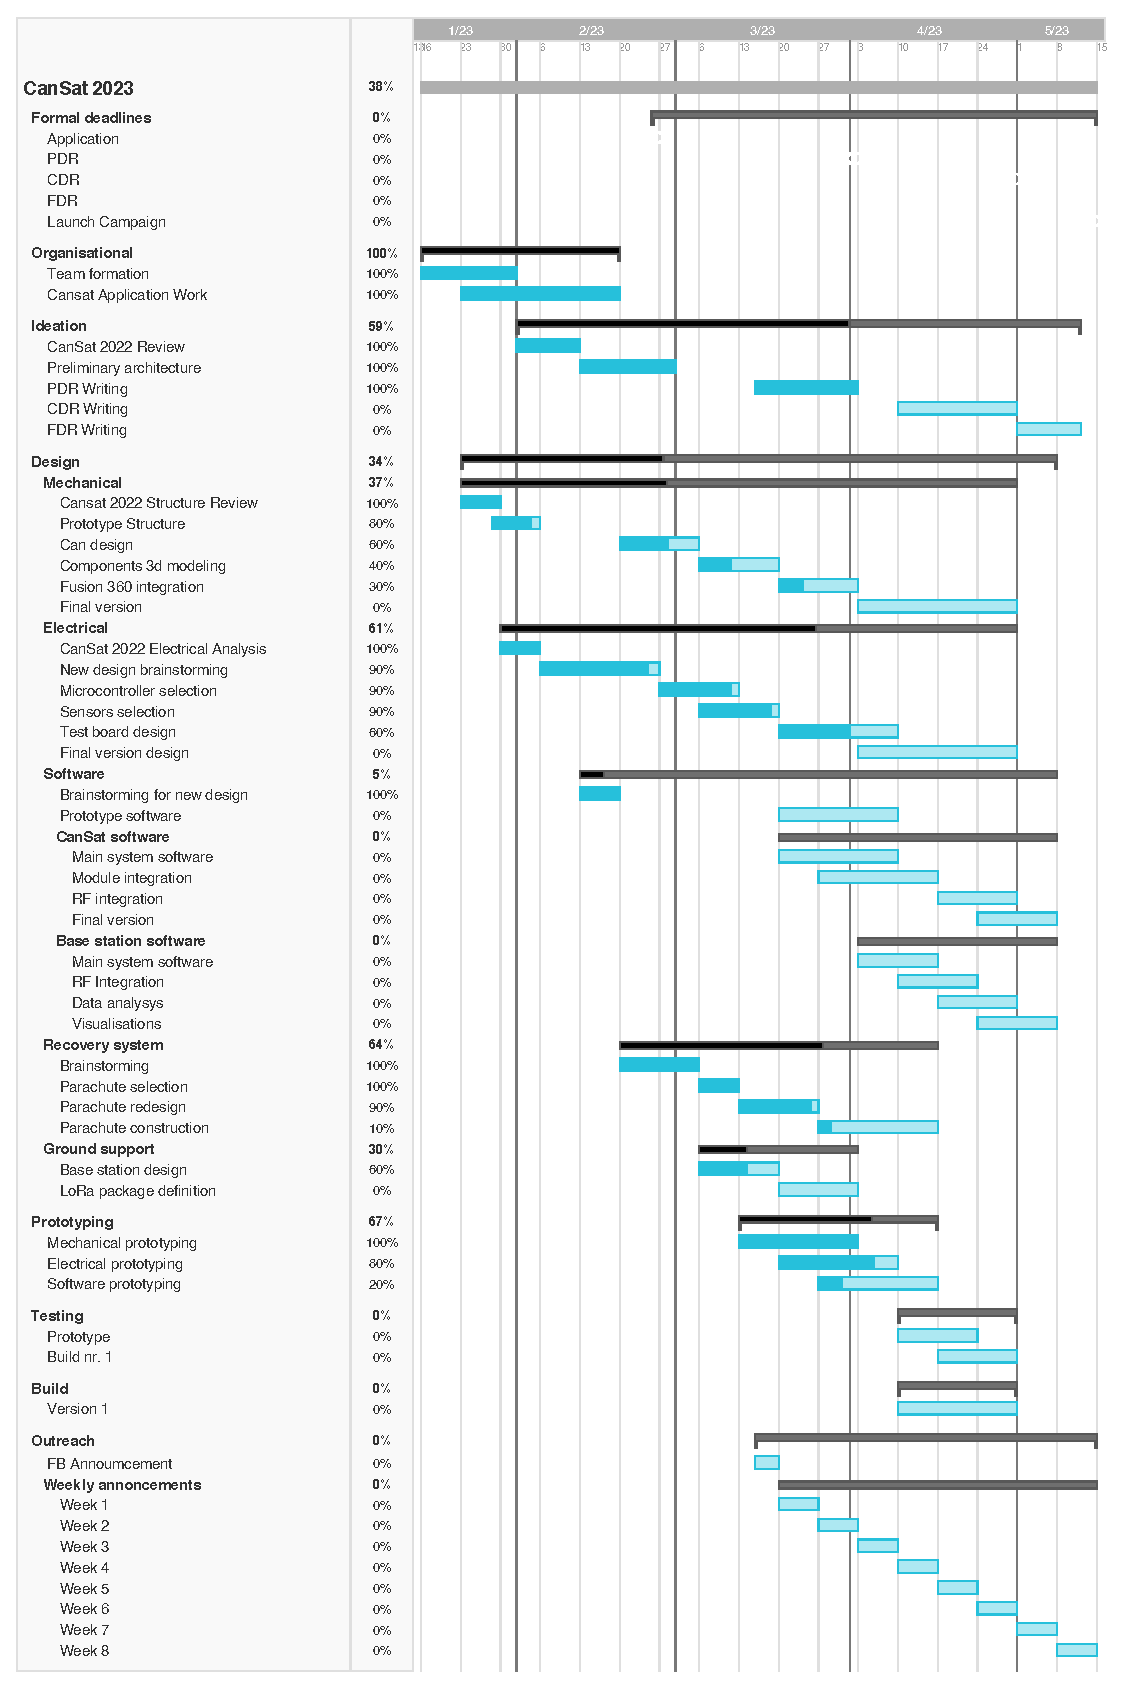
\includegraphics[width=0.9\textwidth]{images/pdr/Gantt.eps}

% Input appendix files
\section{Mission milestones}\label{A33}


These milestones have been designed to keep us on track and ensure that we successfully meet our project goals and deadlines.
\begin{itemize}[leftmargin=1cm, itemindent=0.25cm, noitemsep, topsep=0pt, label=$\bullet$]
    % \item Team Formation and Project Planning:
    % \begin{itemize}[label=\ding{111}, noitemsep, topsep=2pt]
    %     \item Establish team roles and responsibilities
    %     \item Recruit suitable team members for each role
    % \end{itemize}
    \item Define Project Scope and Objectives:
    \begin{itemize}[label=\ding{111}, noitemsep, topsep=0pt]
        \item Purpose of the project: to successfully detect muons and analyze the environment, light conditions
        \item Objectives to be achieved on launch day and post-launch analysis:
        \begin{multicols}{2}
        \setlength{\topsep}{0pt}
        \setlength{\partopsep}{0pt}
        \begin{itemize}[label=\ding{51}, noitemsep, topsep=0pt]
        \item Successful launch
        \item Live RF telemetry
        \item Successful parachute deployment
        \item All systems nominal (good sensor and location data)
        \item Descent rate between 7-10m/s
        \item Landing confirmation
        \item Recovery of the CanSat
        \item Generating reports
        \end{itemize}
        \end{multicols}
    \end{itemize}
    \item Develop a Detailed Project Plan and Timeline:
    \begin{itemize}[label=\ding{111}, noitemsep, topsep=0pt]
        \item Assign tasks related to social media promotion and sponsor search;
        \item Determine cooperation method (online/programs/meetings etc.)
    \end{itemize}
    \item Research and Design:
    \begin{itemize}[label=\ding{111}, noitemsep, topsep=0pt]
        \item Conduct research on required components and technologies for the mission;
        \item Design the payload's structure and select materials;
        \item Submit Preliminary Design Report;
        \item Develop a prototype and test sensors and electronics;
        \item Promote the project on social media platforms and begin searching for sponsors.
    \end{itemize}
    \item Integration and Testing:
    \begin{itemize}[label=\ding{111}, noitemsep, topsep=0pt]
        \item Integrate sensors and electronics into the payload's structure;
        \item Conduct testing and calibration;
        \item Ensure that the CanSat meets weight and size requirements;
    \end{itemize}
    \item Launch Preparation:
    \begin{itemize}[label=\ding{111}, noitemsep, topsep=0pt]
        \item Conduct pre-launch testing;
        \item Pre-launch checklist.
    \end{itemize}
    \item Primary and Secondary Missions:
    \begin{itemize}[label=\ding{111}, noitemsep, topsep=0pt]
        \item Verify that the payload met the primary mission requirements;
        \item Collect the missions data from the sensors;
        \item Conduct data analysis and report on the results;
        \item Share updates and photos of the data analysis on social media platforms.
    \end{itemize}
    \item Submit Design Reviews
    \begin{itemize}[label=\ding{111}, noitemsep, topsep=0pt]
        \item Preliminary Design Review;
        \item Critical Design Review.
    \end{itemize}
    \item Final Report and Presentation:
    \begin{itemize}[label=\ding{111}, noitemsep, topsep=0pt]
    \item Prepare a final report documenting the project's objectives, methods, and results;
    \item Develop a presentation to showcase the mission and its capabilities;
    \item Share the presentation on social media platforms to showcase the project's achievements and thank sponsors for their support.
    \end{itemize}
\end{itemize}
\newpage
\section{Dual parachute design (Payload's Case)}\label{A4}
\coloredbox{CDOSRSecondary!50}{CDOSRPrimary}{CDOSRPrimary}{
    \begin{minipage}{0.4\textwidth}
    The smaller parachute had a diameter of 21.7 cm and a surface area of 370 cm$^{2}$, which is designed to slow down the descent speed to 9 meters per second. The design of this parachute was based on the principles of aerodynamics and is intended to withstand strong winds and turbulent weather conditions. We believe that this parachute will be instrumental in ensuring a safe and successful landing of our Payload during windy weather conditions.
    \end{minipage}
    \hfill
    \begin{minipage}{0.4\textwidth}
    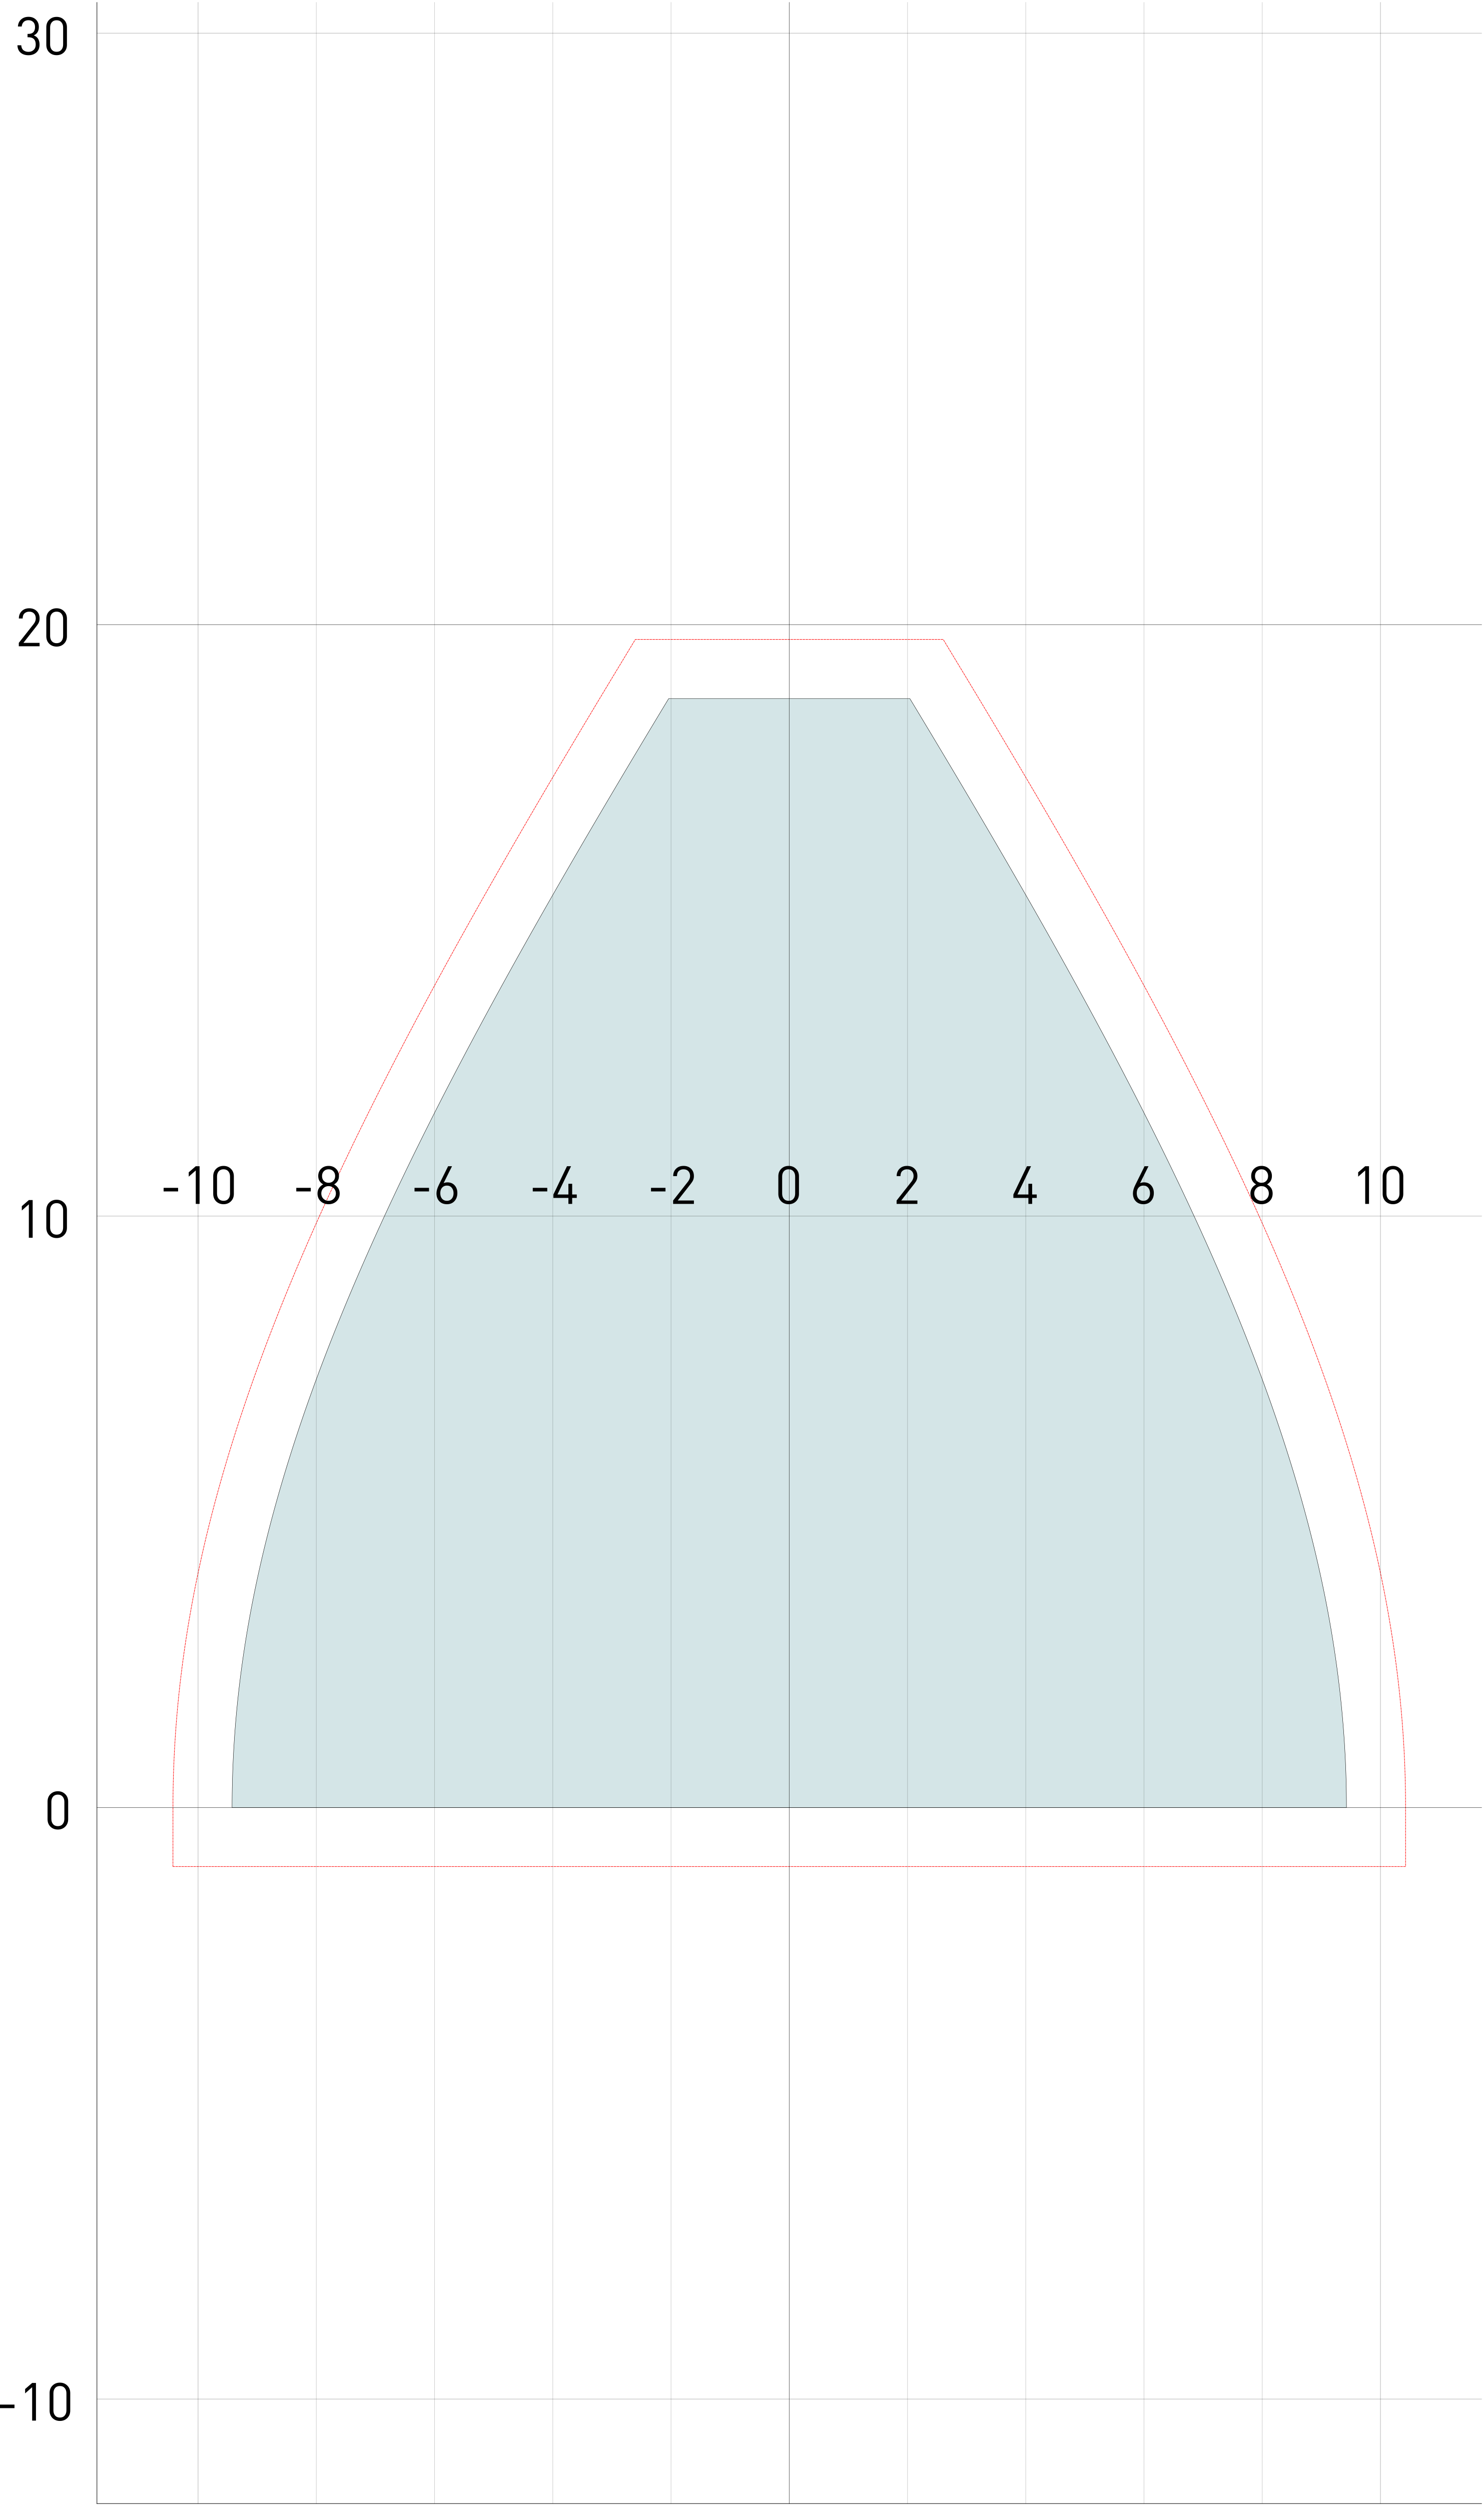
\includegraphics[width=5cm]{PlotItem_2.png}
    \end{minipage}
}
\coloredbox{CDOSRSecondary!50}{CDOSRPrimary}{CDOSRPrimary}{
    \begin{minipage}{0.4\textwidth}
    The second parachute was designed for use during calm weather conditions and had a diameter of 32.6 cm and a surface area of 834 cm$^{2}$, which is designed to slow down the descent speed to 6 meters per second. This parachute was optimized for stable and predictable conditions and is intended to provide a gentle and controlled descent of the Payload during calm weather conditions.
    \end{minipage}
    \hfill
    \begin{minipage}{0.4\textwidth}
    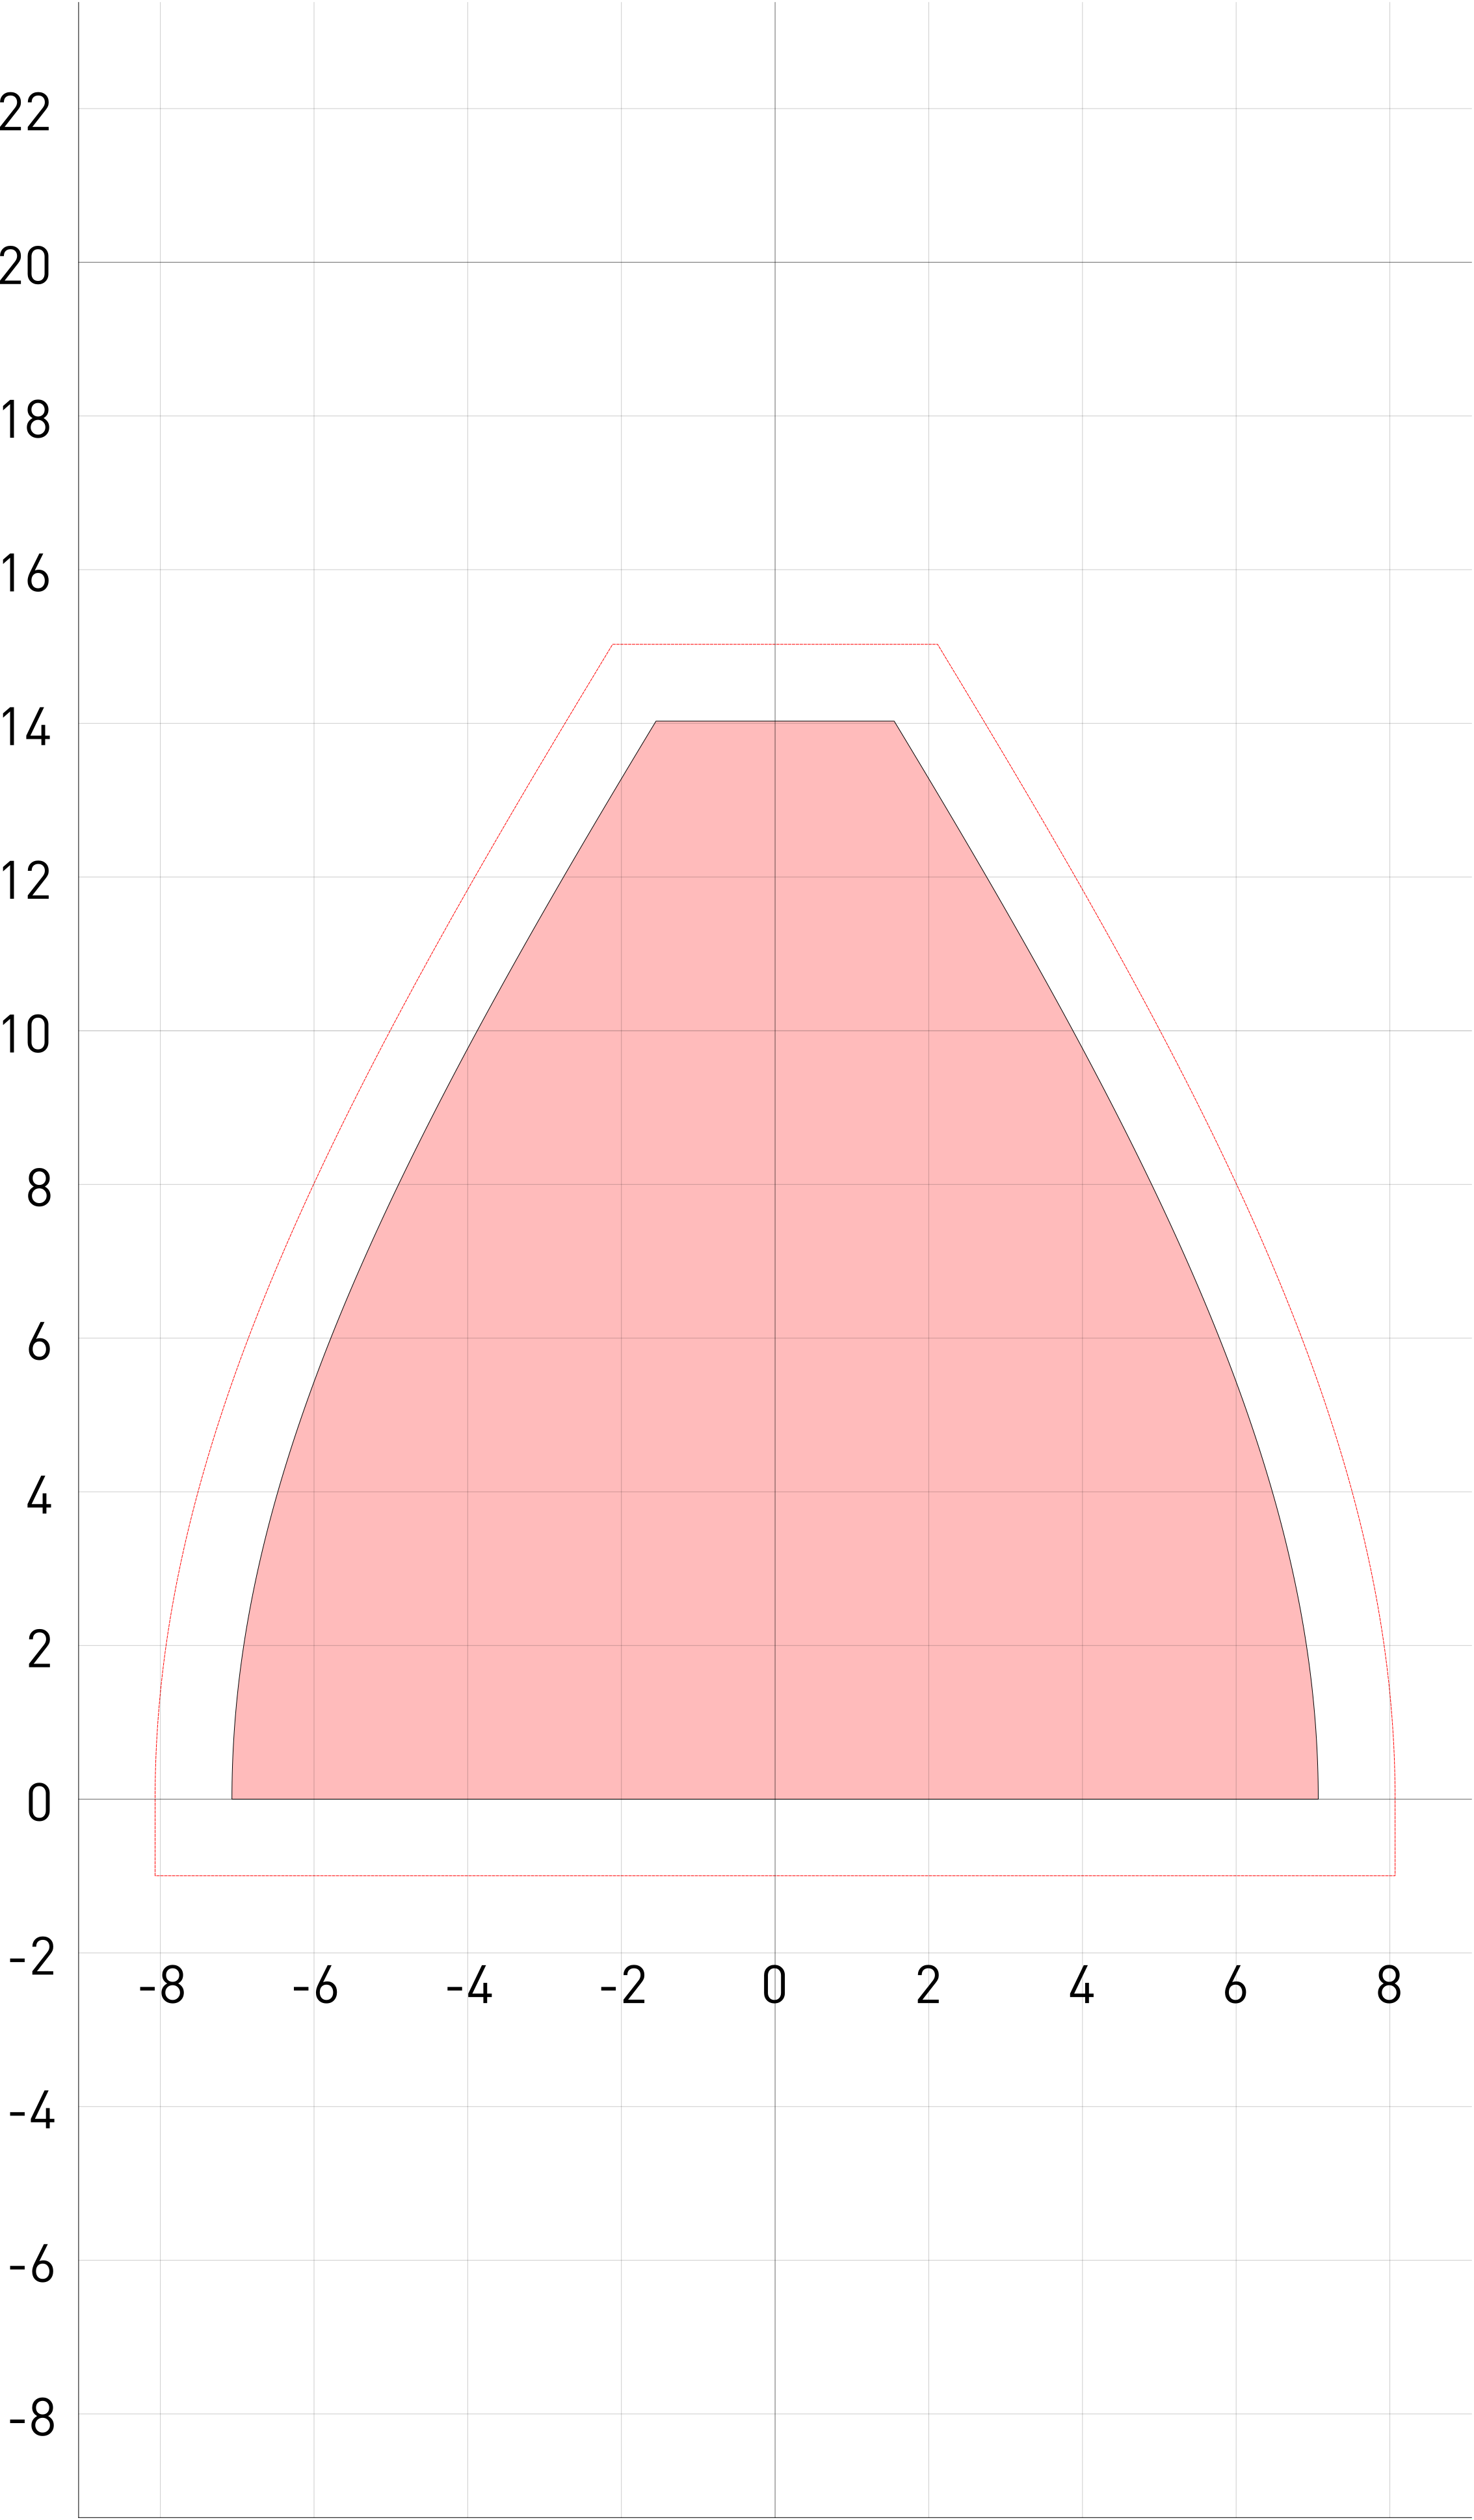
\includegraphics[width=5cm]{PlotItem_1.png}
    \end{minipage}
}
\newpage
\section{Payload  - electrical design}\label{AE2}
% \begin{landscape}
\begin{figure}[h]
    \centering
    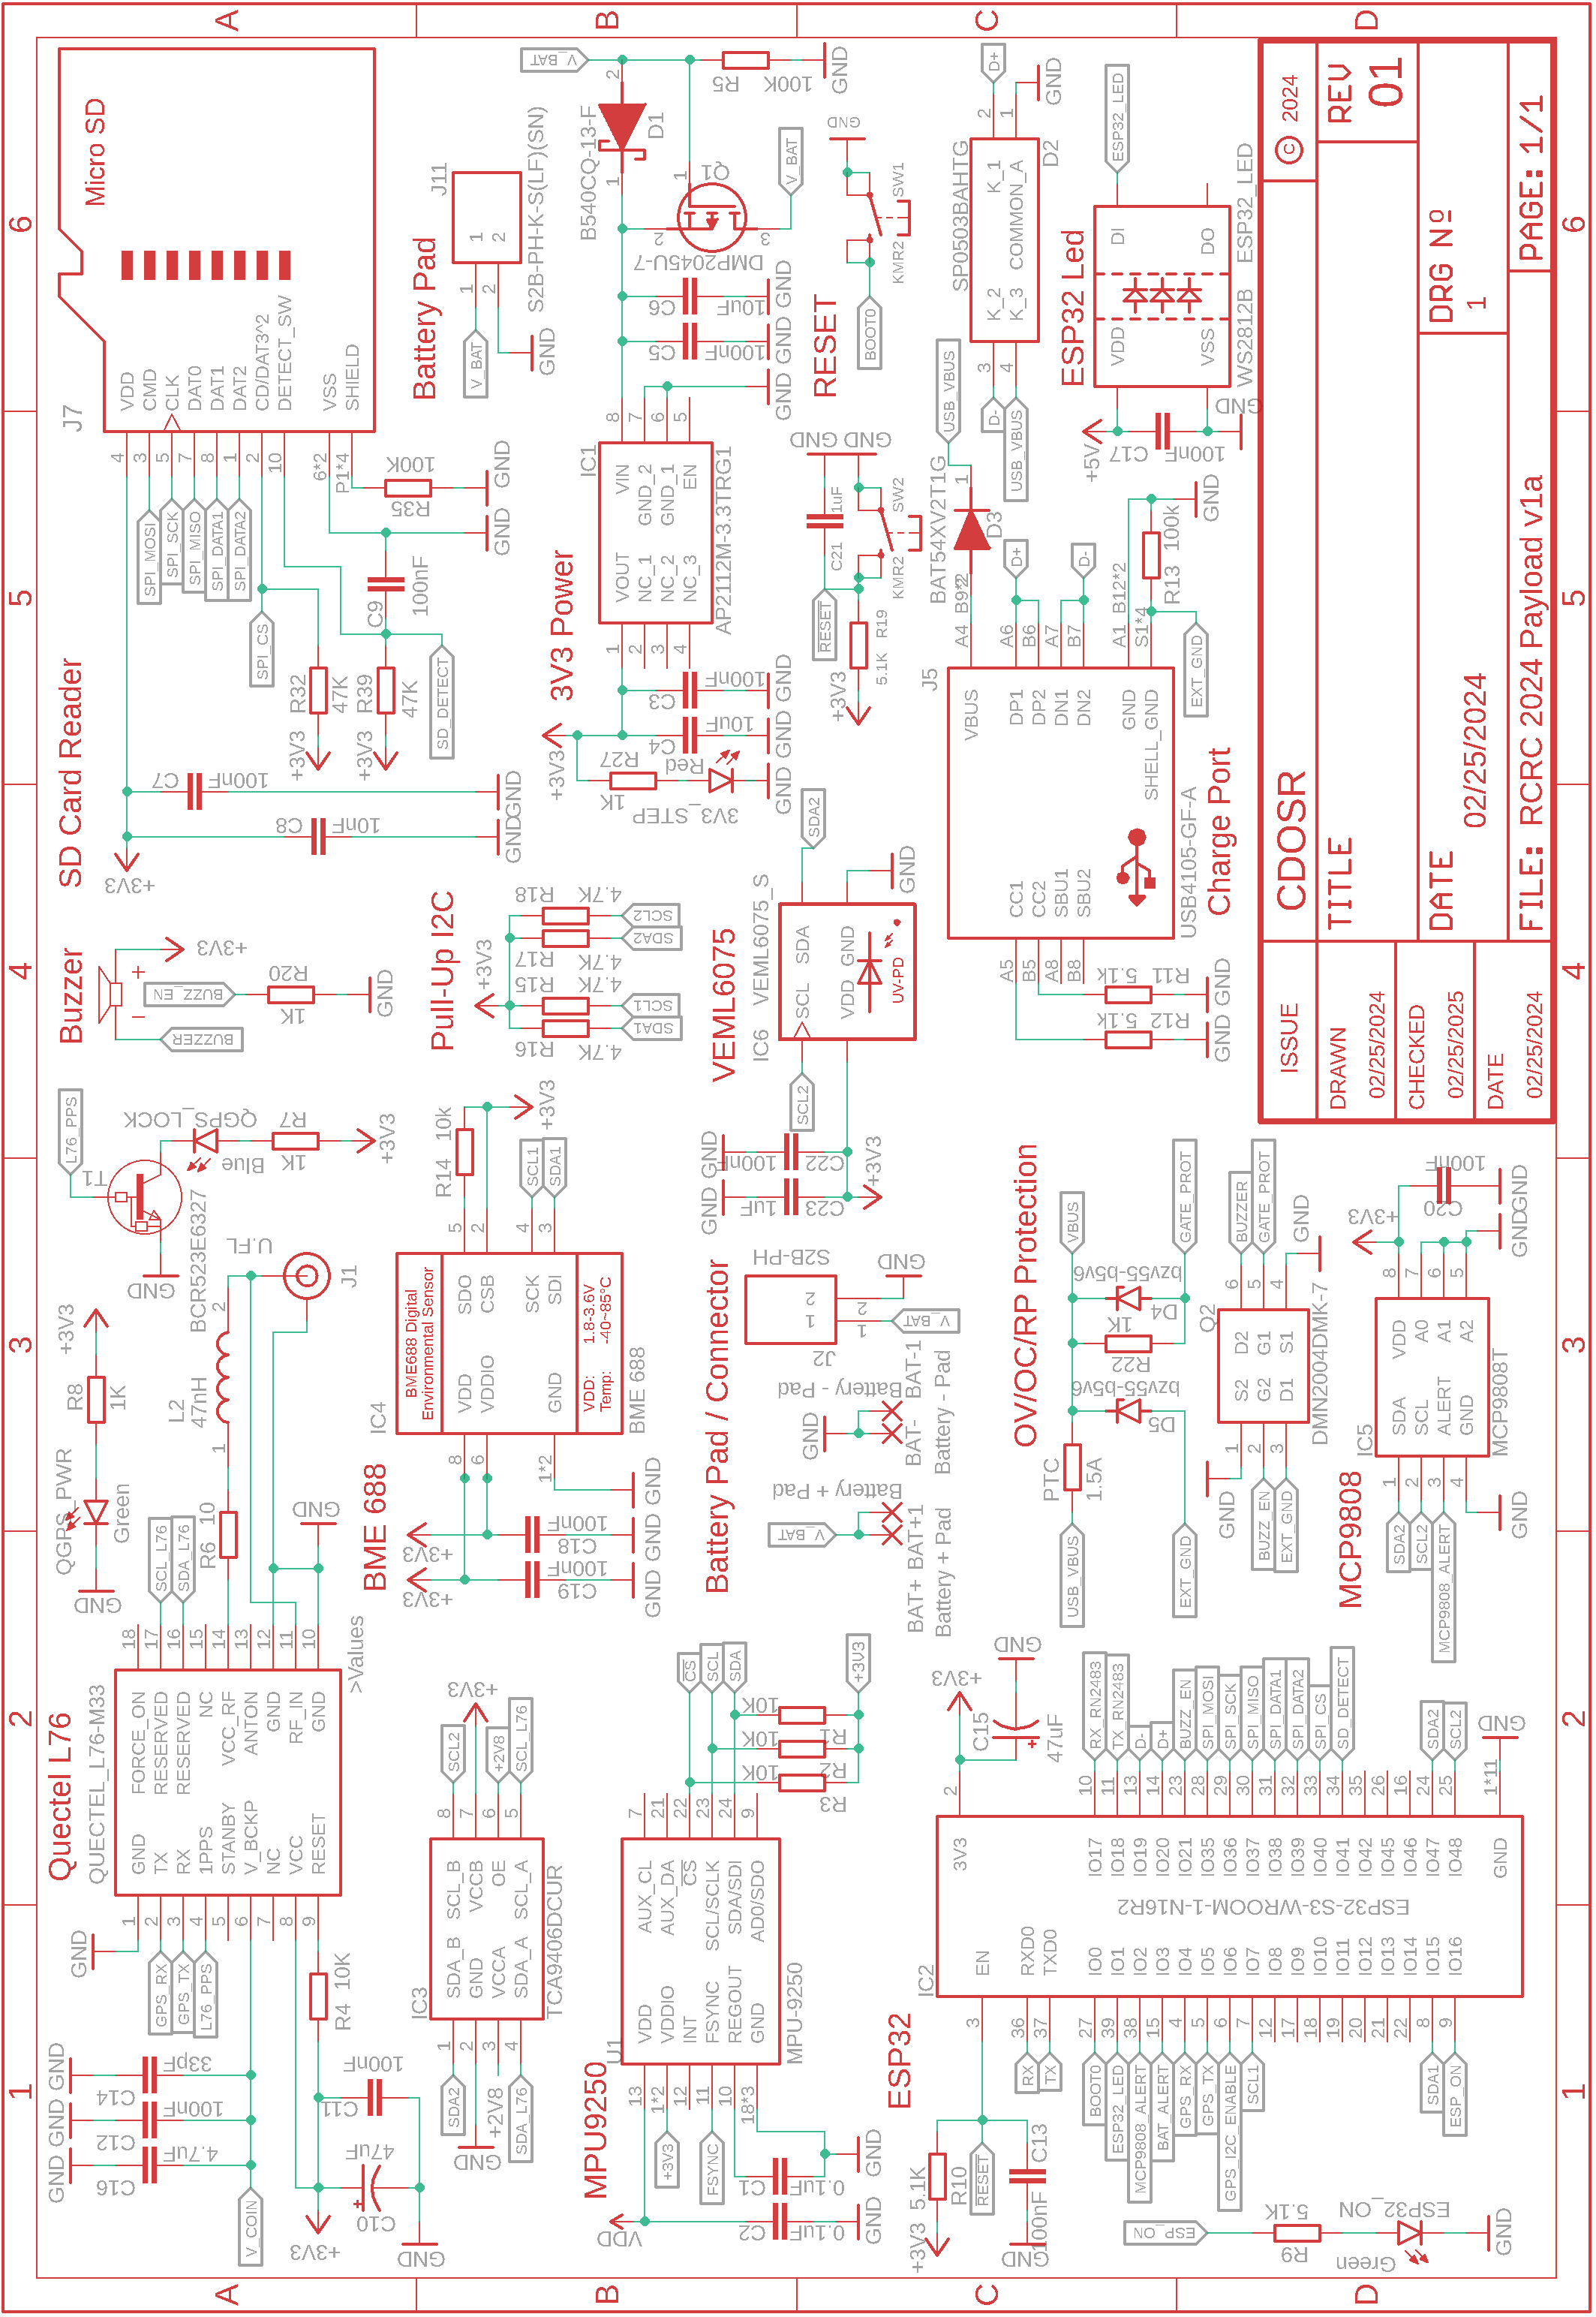
\includegraphics[width=11.4cm]{payload4.png}
    \caption{\small{CDOSR payload electrical scheme.}}
    % \label{fig:gantt}
\end{figure}
% \end{landscape}
\newpage
\section{Base station - electrical design}\label{AEE2}

% \begin{landscape}
\begin{figure}[h]
    \centering
    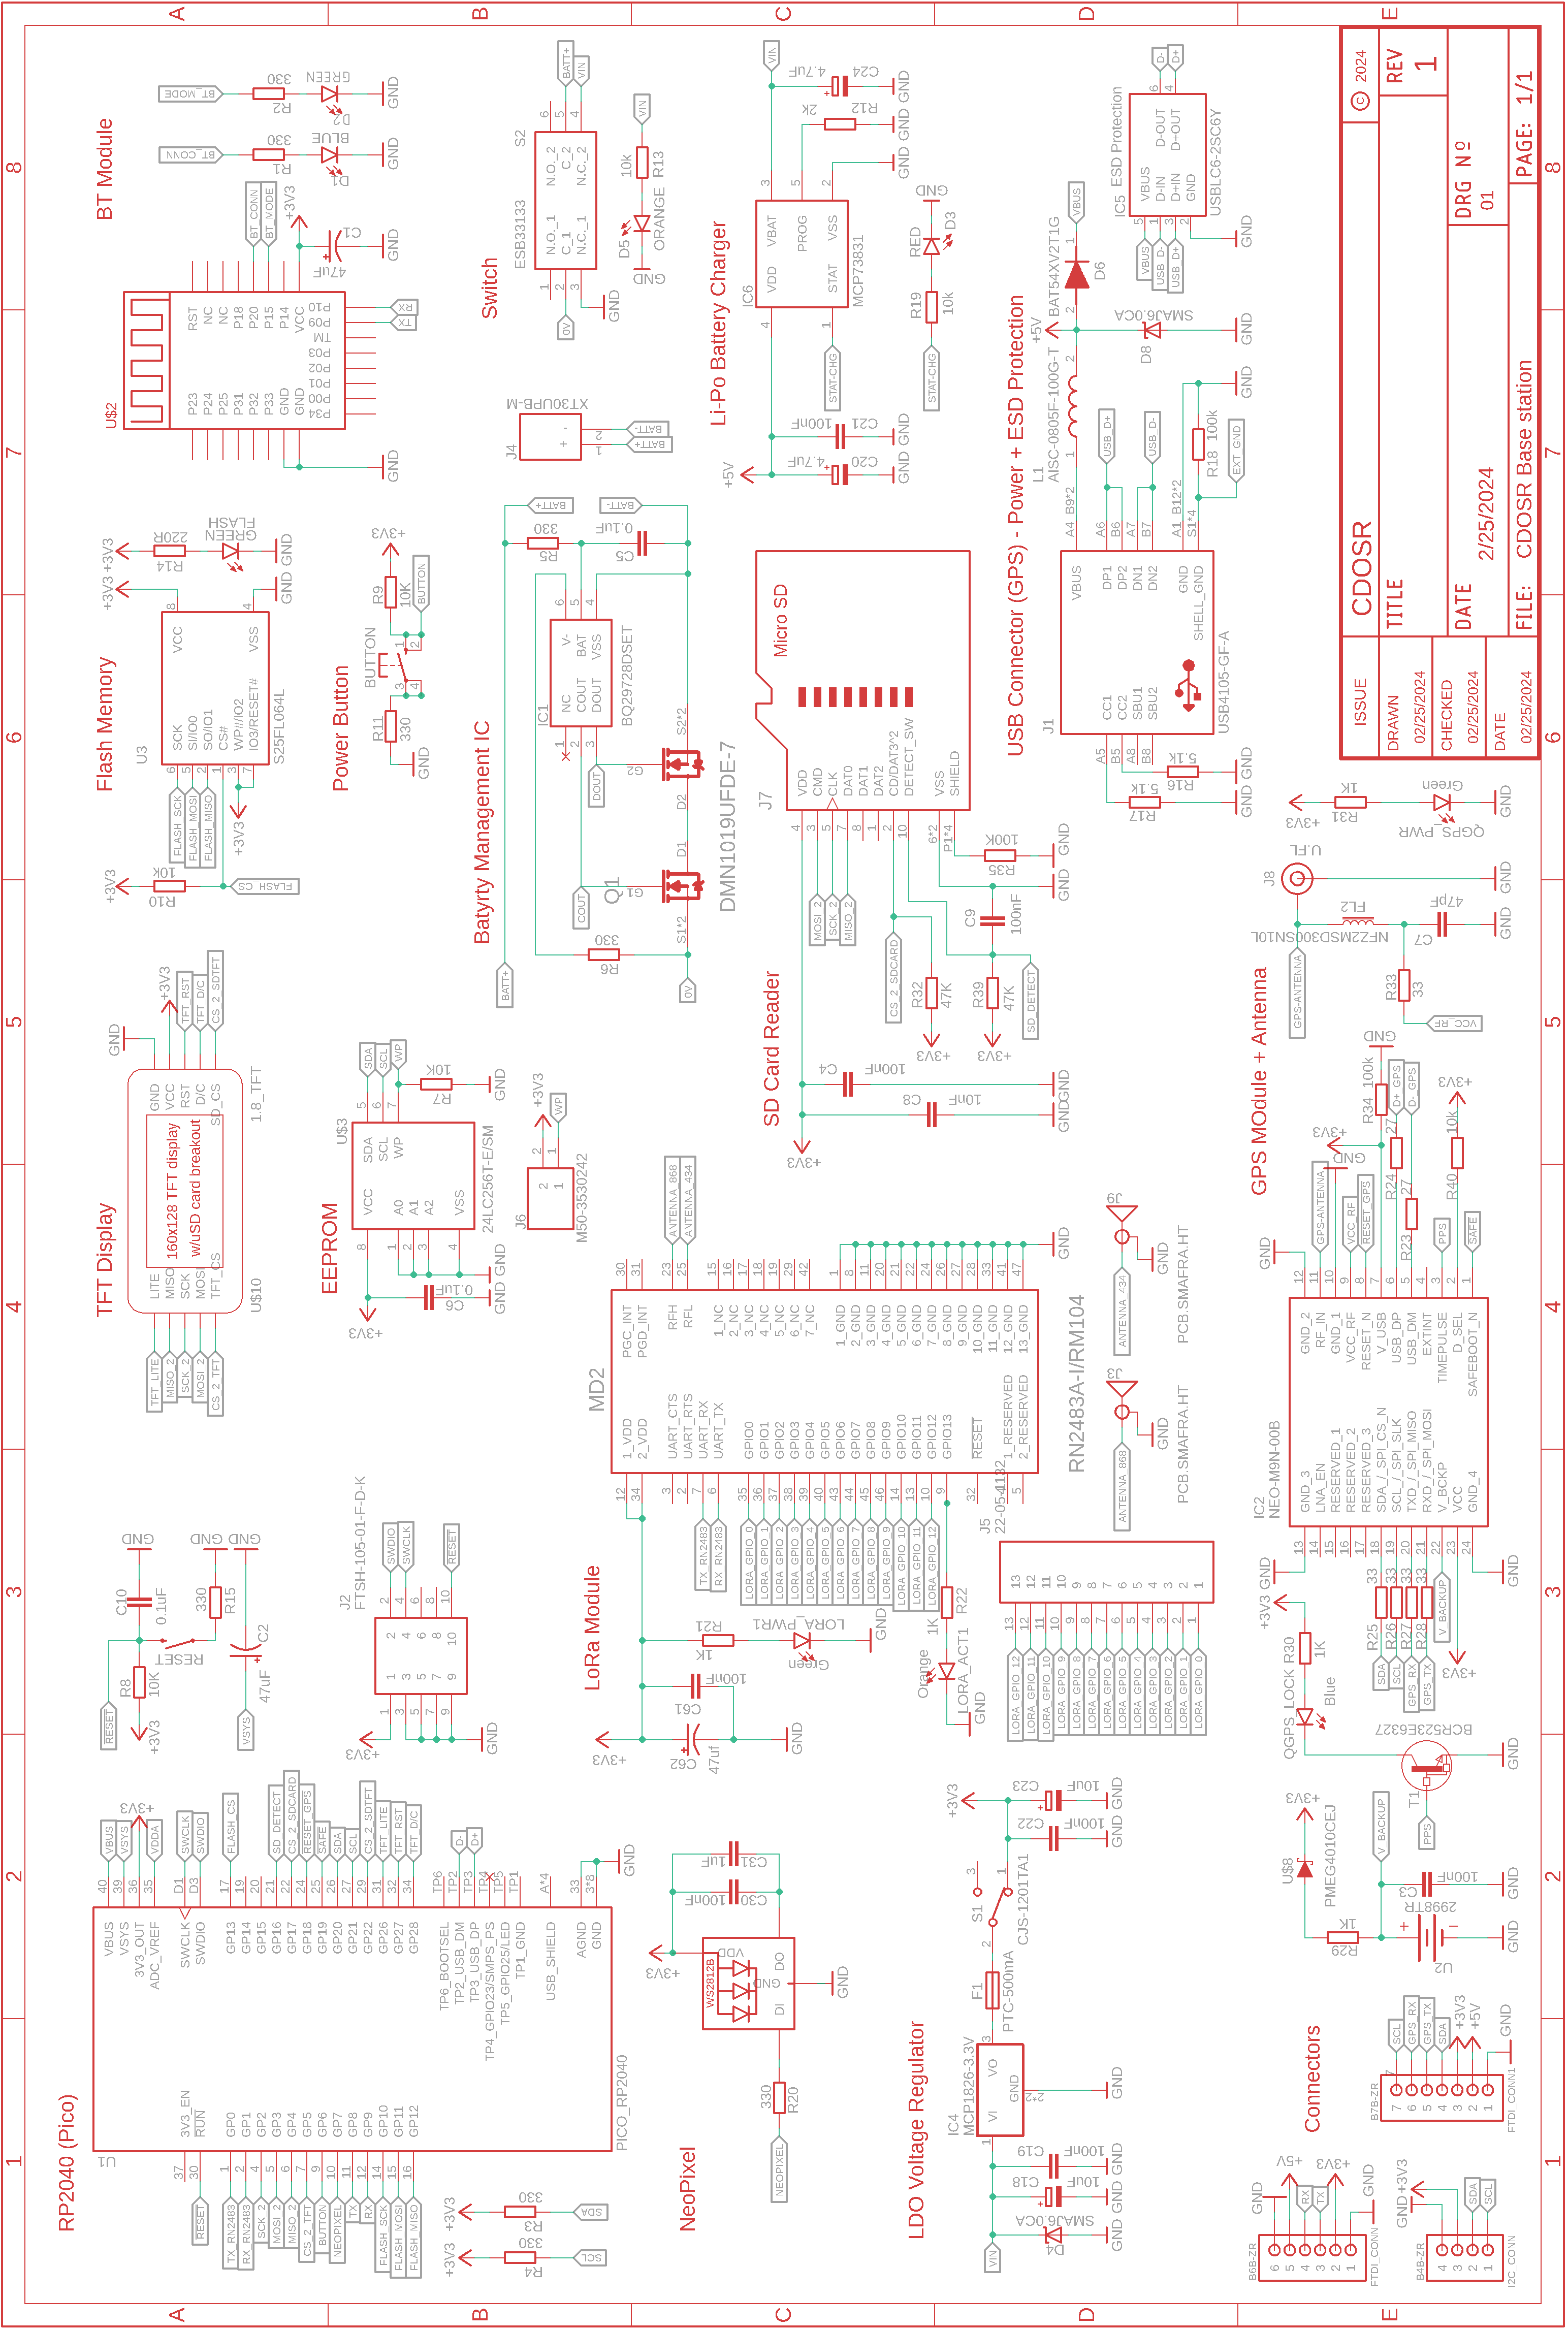
\includegraphics[width=11.4cm]{base_station3.png}
    \caption{\small{CDOSR base station electrical scheme.}}
    % \label{fig:gantt}
\end{figure}
    
% \end{landscape}
\newpage
\section{Test plan}\label{A1}

\begin{itemize}[leftmargin=1cm, itemindent=0.25cm, noitemsep, topsep=0pt, label=\ding{51}]
\item Mission Objective Test
\begin{itemize}[label=\ding{111}, noitemsep, topsep=2pt]
\item Verify if the payload meets the competition mission requirements
\item Check that the sensors are functioning properly
\end{itemize}

\item Mechanical Test
\begin{itemize}[label=\ding{111}, noitemsep, topsep=2pt]
\item Make sure that the structure and enclosure are sturdy and can withstand launch and landing
\item Verify the parachute deployment and fixing are functional and reliable
\end{itemize}

\item Software Test
\begin{itemize}[label=\ding{111}, noitemsep, topsep=2pt]
\item Verify that the software is correctly installed and functional
\item Ensure that the software is properly processing data from the sensors and instruments
\end{itemize}

\item Communication Test
\begin{itemize}[label=\ding{111}, noitemsep, topsep=2pt]
\item Ensure that the payload can communicate with the ground station
\item Verify that telemetry data can be received and decoded correctly
\item Test the range and the reliability of the communication link
\end{itemize}

\item Power Test
\begin{itemize}[label=\ding{111}, noitemsep, topsep=2pt]
\item Verify that the power system meets the power budget and has sufficient power to operate the payload
\item Test the duration of the battery life and ensure that power consumption is minimized wherever possible
\end{itemize}

\item Integration Test
\begin{itemize}[label=\ding{111}, noitemsep, topsep=2pt]
\item Verify if all the components of the payload are properly integrated and functioning correctly
\item Test the overall functionality
\end{itemize}

\item Ground Station Test
\begin{itemize}[label=\ding{111}, noitemsep, topsep=2pt]
\item Verify that the antennas are properly installed and functional
\item Verify that the ground station software can display data from the payload
\end{itemize}

\item Battery Charging Test
\begin{itemize}[label=\ding{111}, noitemsep, topsep=2pt]
\item Test the battery charging system and verify that it can fully charge the batteries within a reasonable amount of time
\item Verify that the charging system is safe and reliable
\end{itemize}

\item Post-Mission Test
\begin{itemize}[label=\ding{111}, noitemsep, topsep=2pt]
\item Verify if the payload has returned all the required data
\item Check the data for accuracy and completeness
\item Analyze the data and compare it to the mission objectives
\end{itemize}

\end{itemize}
\newpage
\section{Sensor testing}\label{A22}

\begin{itemize}[labelwidth=0cm, leftmargin=0cm, itemindent=0.7cm, noitemsep, topsep=0pt, label={}]
\item \textbf{Pressure sensor test}:
\begin{itemize}[labelwidth=2cm, leftmargin=1.9cm, label=\ding{109}, noitemsep, topsep=2pt]
\item[\faTasks] \textbf{Task}: Expose the used sensor to a pressure change and compare the results with a reference device.
\item[\faFlask] \textbf{Method}: Place the target and reference sensors in a sealed container with a known volume of air and measure the pressure change with a manometer or a barometer. The pressure can be changed by altering the volume of the container or by using a hand pump.
\item[{\faHourglass[3]}] \textbf{Estimated testing time duration}: 1-2 hours
\item[{\faCheckSquare}] \textbf{Acceptance criteria}: The test will be considered positive when both sensors show the same pressure without measuring errors.
\end{itemize}
\item \textbf{Temperature sensor test}:
\begin{itemize}[labelwidth=2cm, leftmargin=1.9cm, label=\ding{109}, noitemsep, topsep=2pt]
\item[\faTasks] \textbf{Task}:  Check whether the target device and the reference device show the same temperature within 24 hours 
\item[\faFlask] \textbf{Method}: Place both the target device and the reference device in the same location and monitor their temperature readings at regular intervals for 24 hours
\item[{\faHourglass[3]}] \textbf{Estimated testing time duration}:  24 hours
\item[{\faCheckSquare}] \textbf{Acceptance criteria}: The test will be considered positive when both sensors show the same temperature without significant deviation.
\end{itemize}
\item \textbf{Humidity sensor test}:
\begin{itemize}[labelwidth=2cm, leftmargin=1.9cm, label=\ding{109}, noitemsep, topsep=2pt]
\item[\faTasks] \textbf{Task}:  Place the target sensor and the reference device in a humidity chamber where the humidity will be increased or decreased to a specific level, and the readings will be compared.
\item[\faFlask] \textbf{Method}: The target sensor and the reference device will be placed in a humidity chamber where the humidity level will be gradually increased or decreased to a specific level. The readings from both sensors will be recorded and compared.
\item[{\faHourglass[3]}] \textbf{Estimated testing time duration}:  6 hours
\item[{\faCheckSquare}] \textbf{Acceptance criteria}: The test will be considered positive when both sensors show the same humidity level without significant deviation.
\end{itemize}
\item \textbf{UV sensor test}:
\begin{itemize}[labelwidth=2cm, leftmargin=1.9cm, label=\ding{109}, noitemsep, topsep=2pt]
\item[\faTasks] \textbf{Task}:  Expose the target sensor and the reference device to UV radiation from a UV light source and compare the readings.
\item[\faFlask] \textbf{Method}: The target sensor and the reference device will be exposed to UV radiation from a UV light source for a specific duration, and the readings will be recorded and compared.
\item[{\faHourglass[3]}] \textbf{Estimated testing time duration}:  1 hour
\item[{\faCheckSquare}] \textbf{Acceptance criteria}: The test will be considered positive when both sensors show the same UV index without significant deviation.
\end{itemize}
\item \textbf{GPS test}:
\begin{itemize}[labelwidth=2cm, leftmargin=1.9cm, label=\ding{109}, noitemsep, topsep=2pt]
\item[\faTasks] \textbf{Task}:  Test the accuracy of the GPS module by comparing the location obtained by the CanSat with the actual location.
\item[\faFlask] \textbf{Method}: The location data collected by the GPS module during this time will be recorded and compared to the actual location using a separate reference system. The reference system may be a ground-based GPS receiver or a separate device with accurate location data.
\item[{\faHourglass[3]}] \textbf{Estimated testing time duration}:  1 hour
\item[{\faCheckSquare}] \textbf{Acceptance criteria}: The test will be considered positive if the error margin is within an acceptable range.
\end{itemize}
\end{itemize}

\newpage
\section{Mechanical stress testing}\label{A33333}


\begin{itemize}[labelwidth=0cm, leftmargin=0cm, itemindent=0.7cm, noitemsep, topsep=0pt, label={}]
\item \textbf{Drop resistance test}:
\begin{itemize}[labelwidth=2cm, leftmargin=1.9cm, label=\ding{109}, noitemsep, topsep=2pt]
\item[\faTasks] \textbf{Task}: Conduct a crash test to ensure the payload components can withstand the impact of a fall.
\item[\faFlask] \textbf{Method}: Prototypes will be dropped from a tower or drone to achieve the required descent speed. A fall test without a parachute will also be performed. Optionally, a 3-axis accelerometer will be added to record any G-force during the test.
\item[{\faHourglass[3]}] \textbf{Estimated testing time duration}: Estimated to be a few hours.
\item[{\faCheckSquare}] \textbf{Acceptance criteria}: All components should remain intact, and the electronics should continue to work continuously.
\end{itemize}
\item \textbf{Long-term G-force tests}:
\begin{itemize}[labelwidth=2cm, leftmargin=1.9cm, label=\ding{109}, noitemsep, topsep=2pt]
\item[\faTasks] \textbf{Task}: Simulate the G-forces that may occur during rocket transport to test the CanSat components' endurance.
\item[\faFlask] \textbf{Method}: The payload model will be placed on a carousel or string and rapidly rotated to generate the required overload due to the centrifugal force.
\item[{\faHourglass[3]}] \textbf{Estimated testing time duration}: The test will last for several hours.
\item[{\faCheckSquare}] \textbf{Acceptance criteria}: All components should remain intact, and the electronics should continue to work continuously throughout the test period.
\end{itemize}
\end{itemize}

\printglossary[type=\acronymtype,title=Acronyms]
\printglossary[title=Glossary]


\end{document}
